




\section{time analysis}
This section is based on the commit "Interactive with time measurement".

\begin{figure}[h]
	\centering
	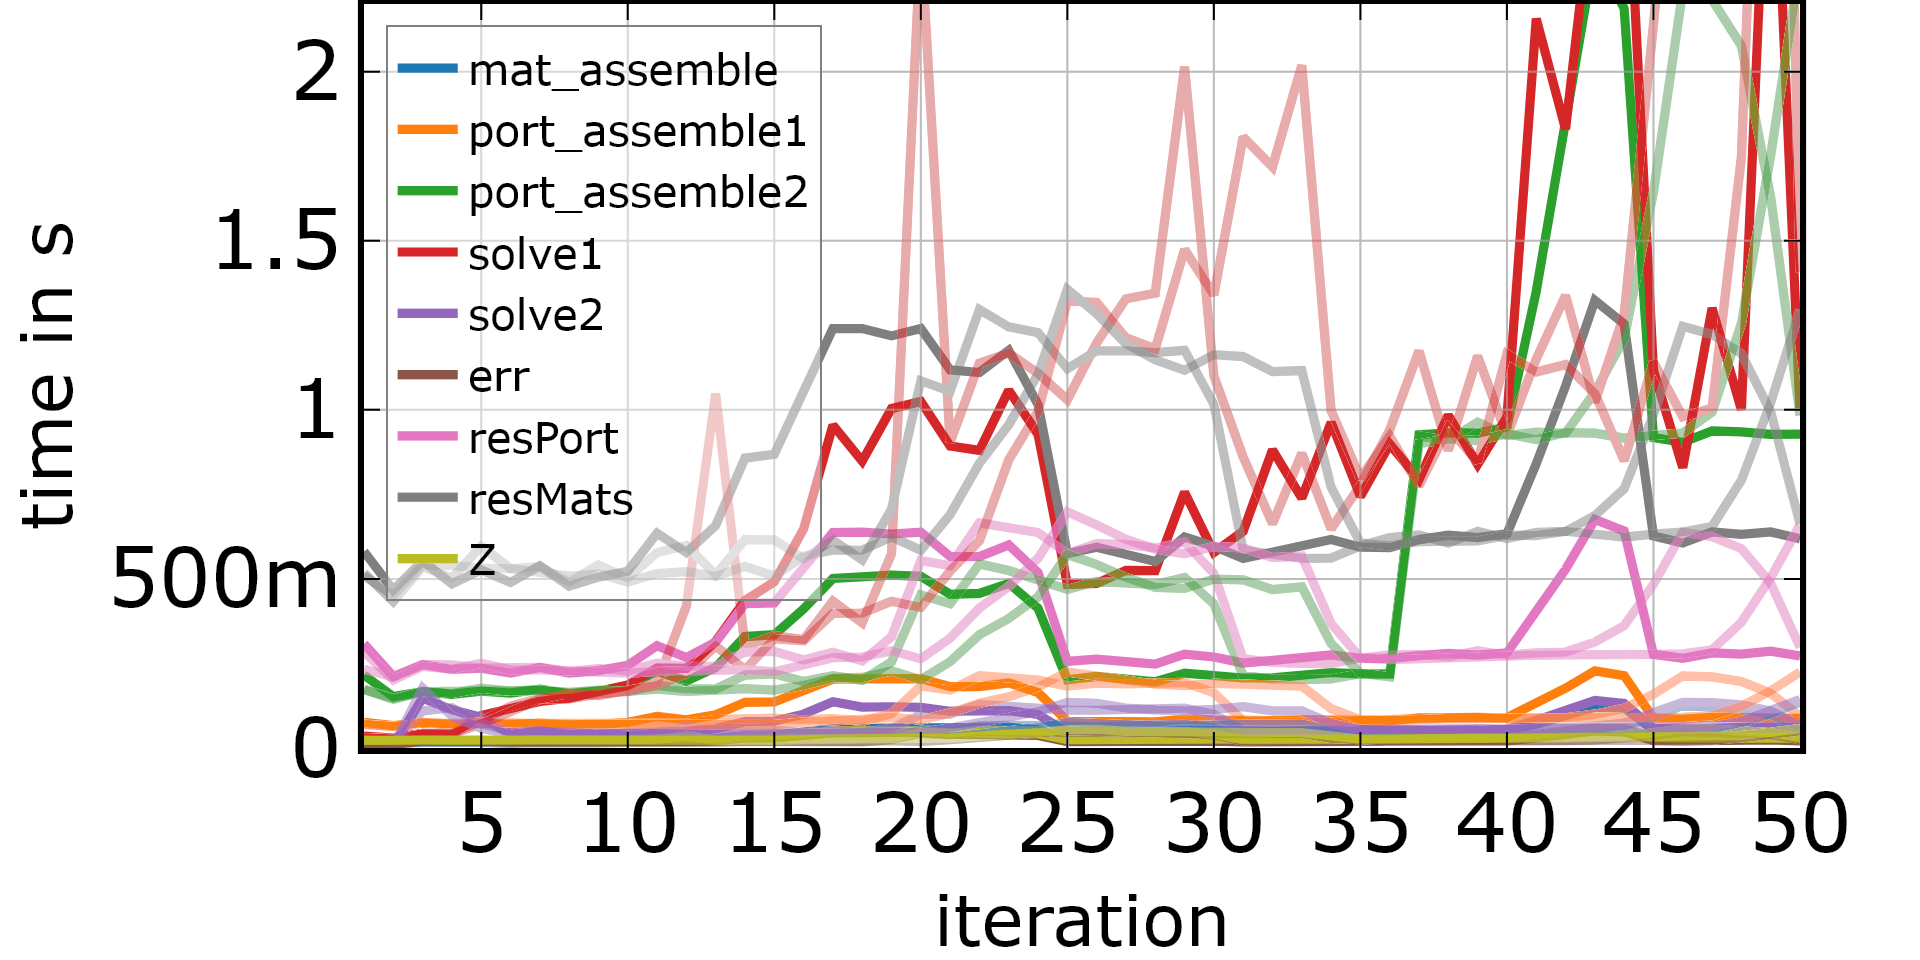
\includegraphics[width=0.5\textwidth]{CubeWire_time_merge1.PNG}
	\caption{Three runtimes for the Cubewire. The opaque lines show one run, the transparent ones two further ones. The increases at around iteration 20 and 40 are likely due to the cooling/turbo boost of the laptop, which can be confirmed by monitoring the task manager. Occasional spikes are distributed randomly, so likely caused by background processes. Important is the sudden increase of port-assemble2 at iteration 37 in all three runs. Also important is solve1, since it is the one which is increasing the quickest.}
	\label{}
\end{figure}


\begin{figure}[h]
	\centering
	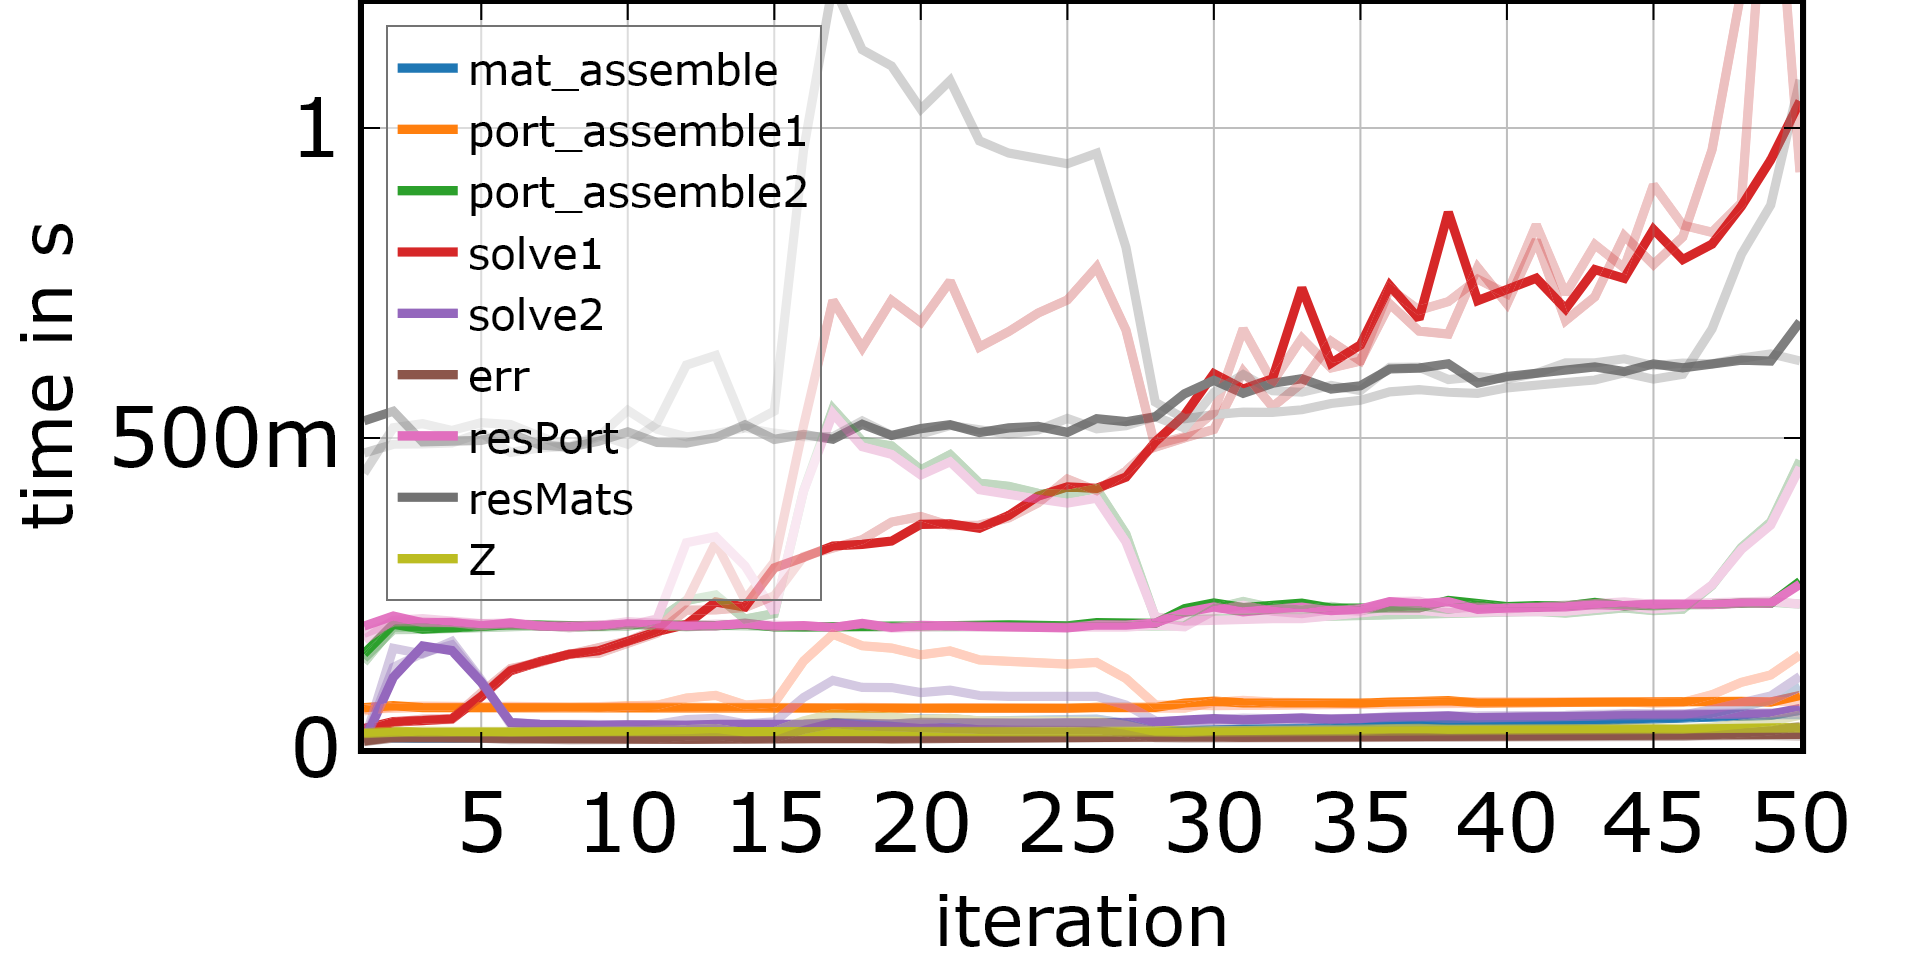
\includegraphics[width=0.5\textwidth]{sqav_time_merge1.PNG}
	\caption{Three runtimes for the square cavity. The opaque lines show one run, the transparent ones two further ones. Similar results as for the cube wire}
	\label{}
\end{figure}



\begin{figure}[h]
	\centering
	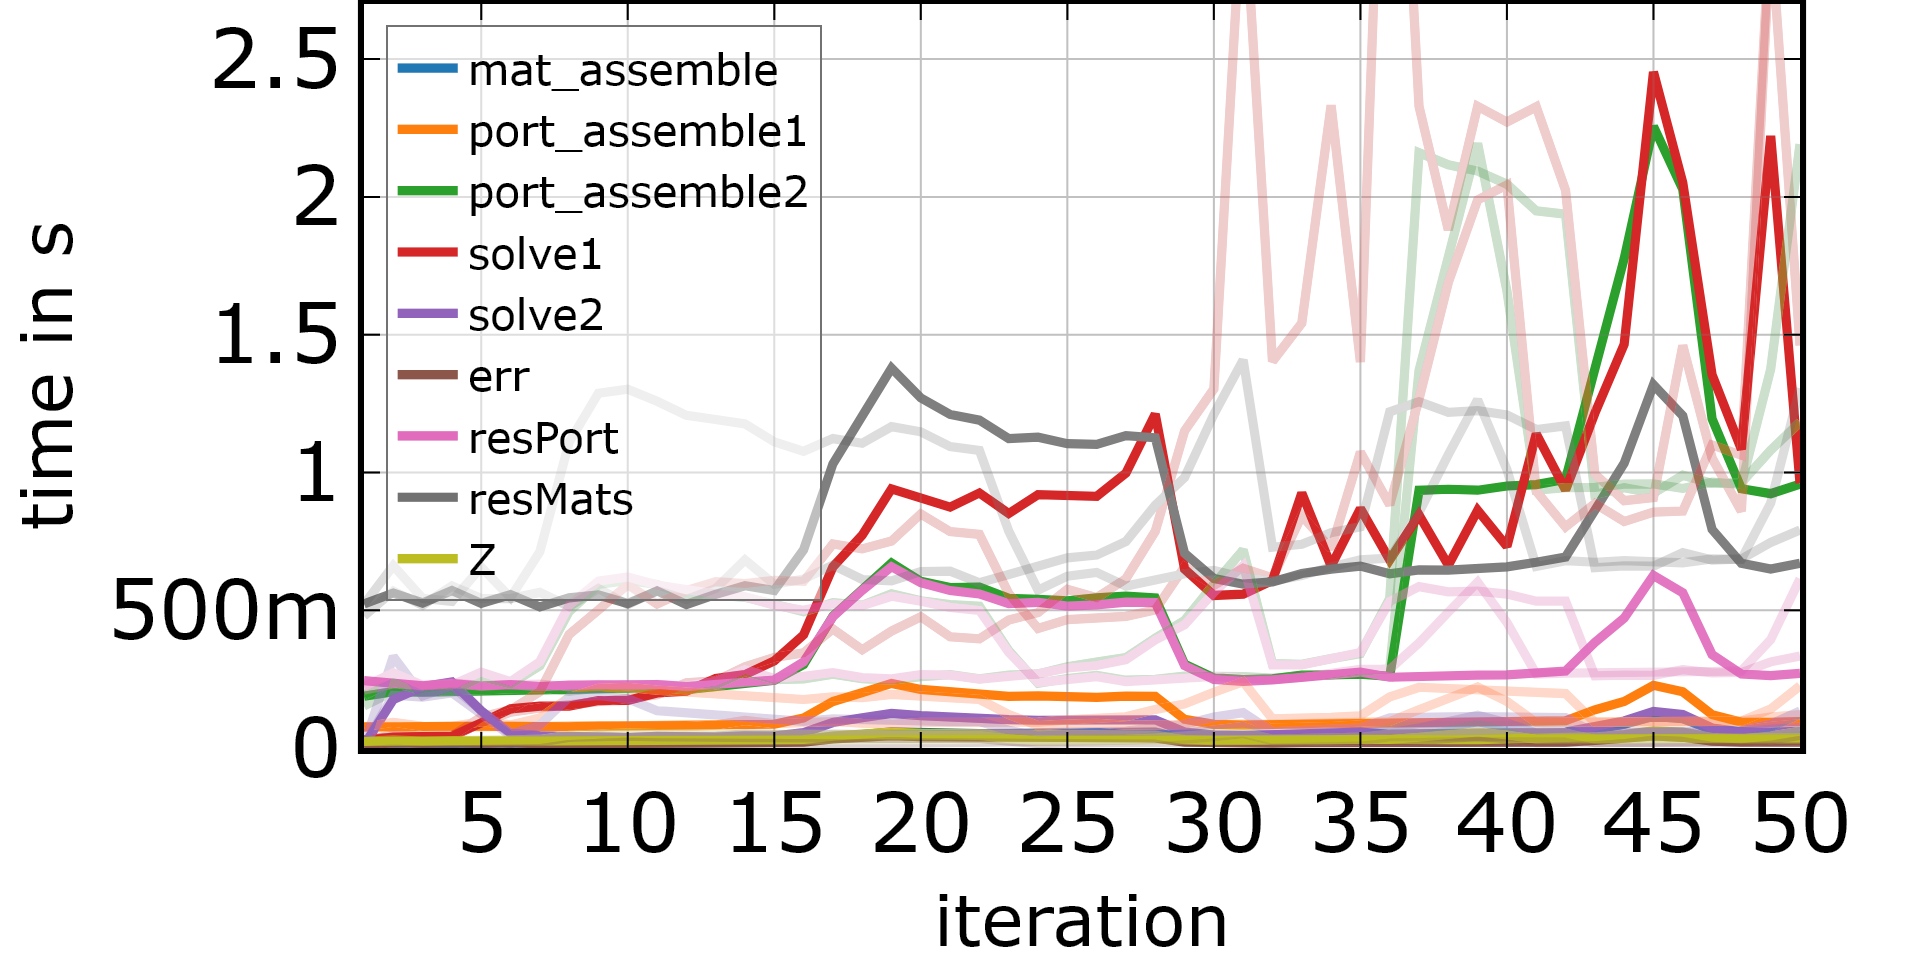
\includegraphics[width=0.5\textwidth]{const_time_merge1.PNG}
	\caption{Three runtimes for the constriction. The opaque lines show one run, the transparent ones two further ones. Similar results as for the cube wire. Here is also a sudden increase of port-assemble2 at iteration 37 in all three runs.}
	\label{}
\end{figure}

\subsection{Accelerator Cavity with 20.5k Nodes}
\begin{figure}[h]
	\centering
	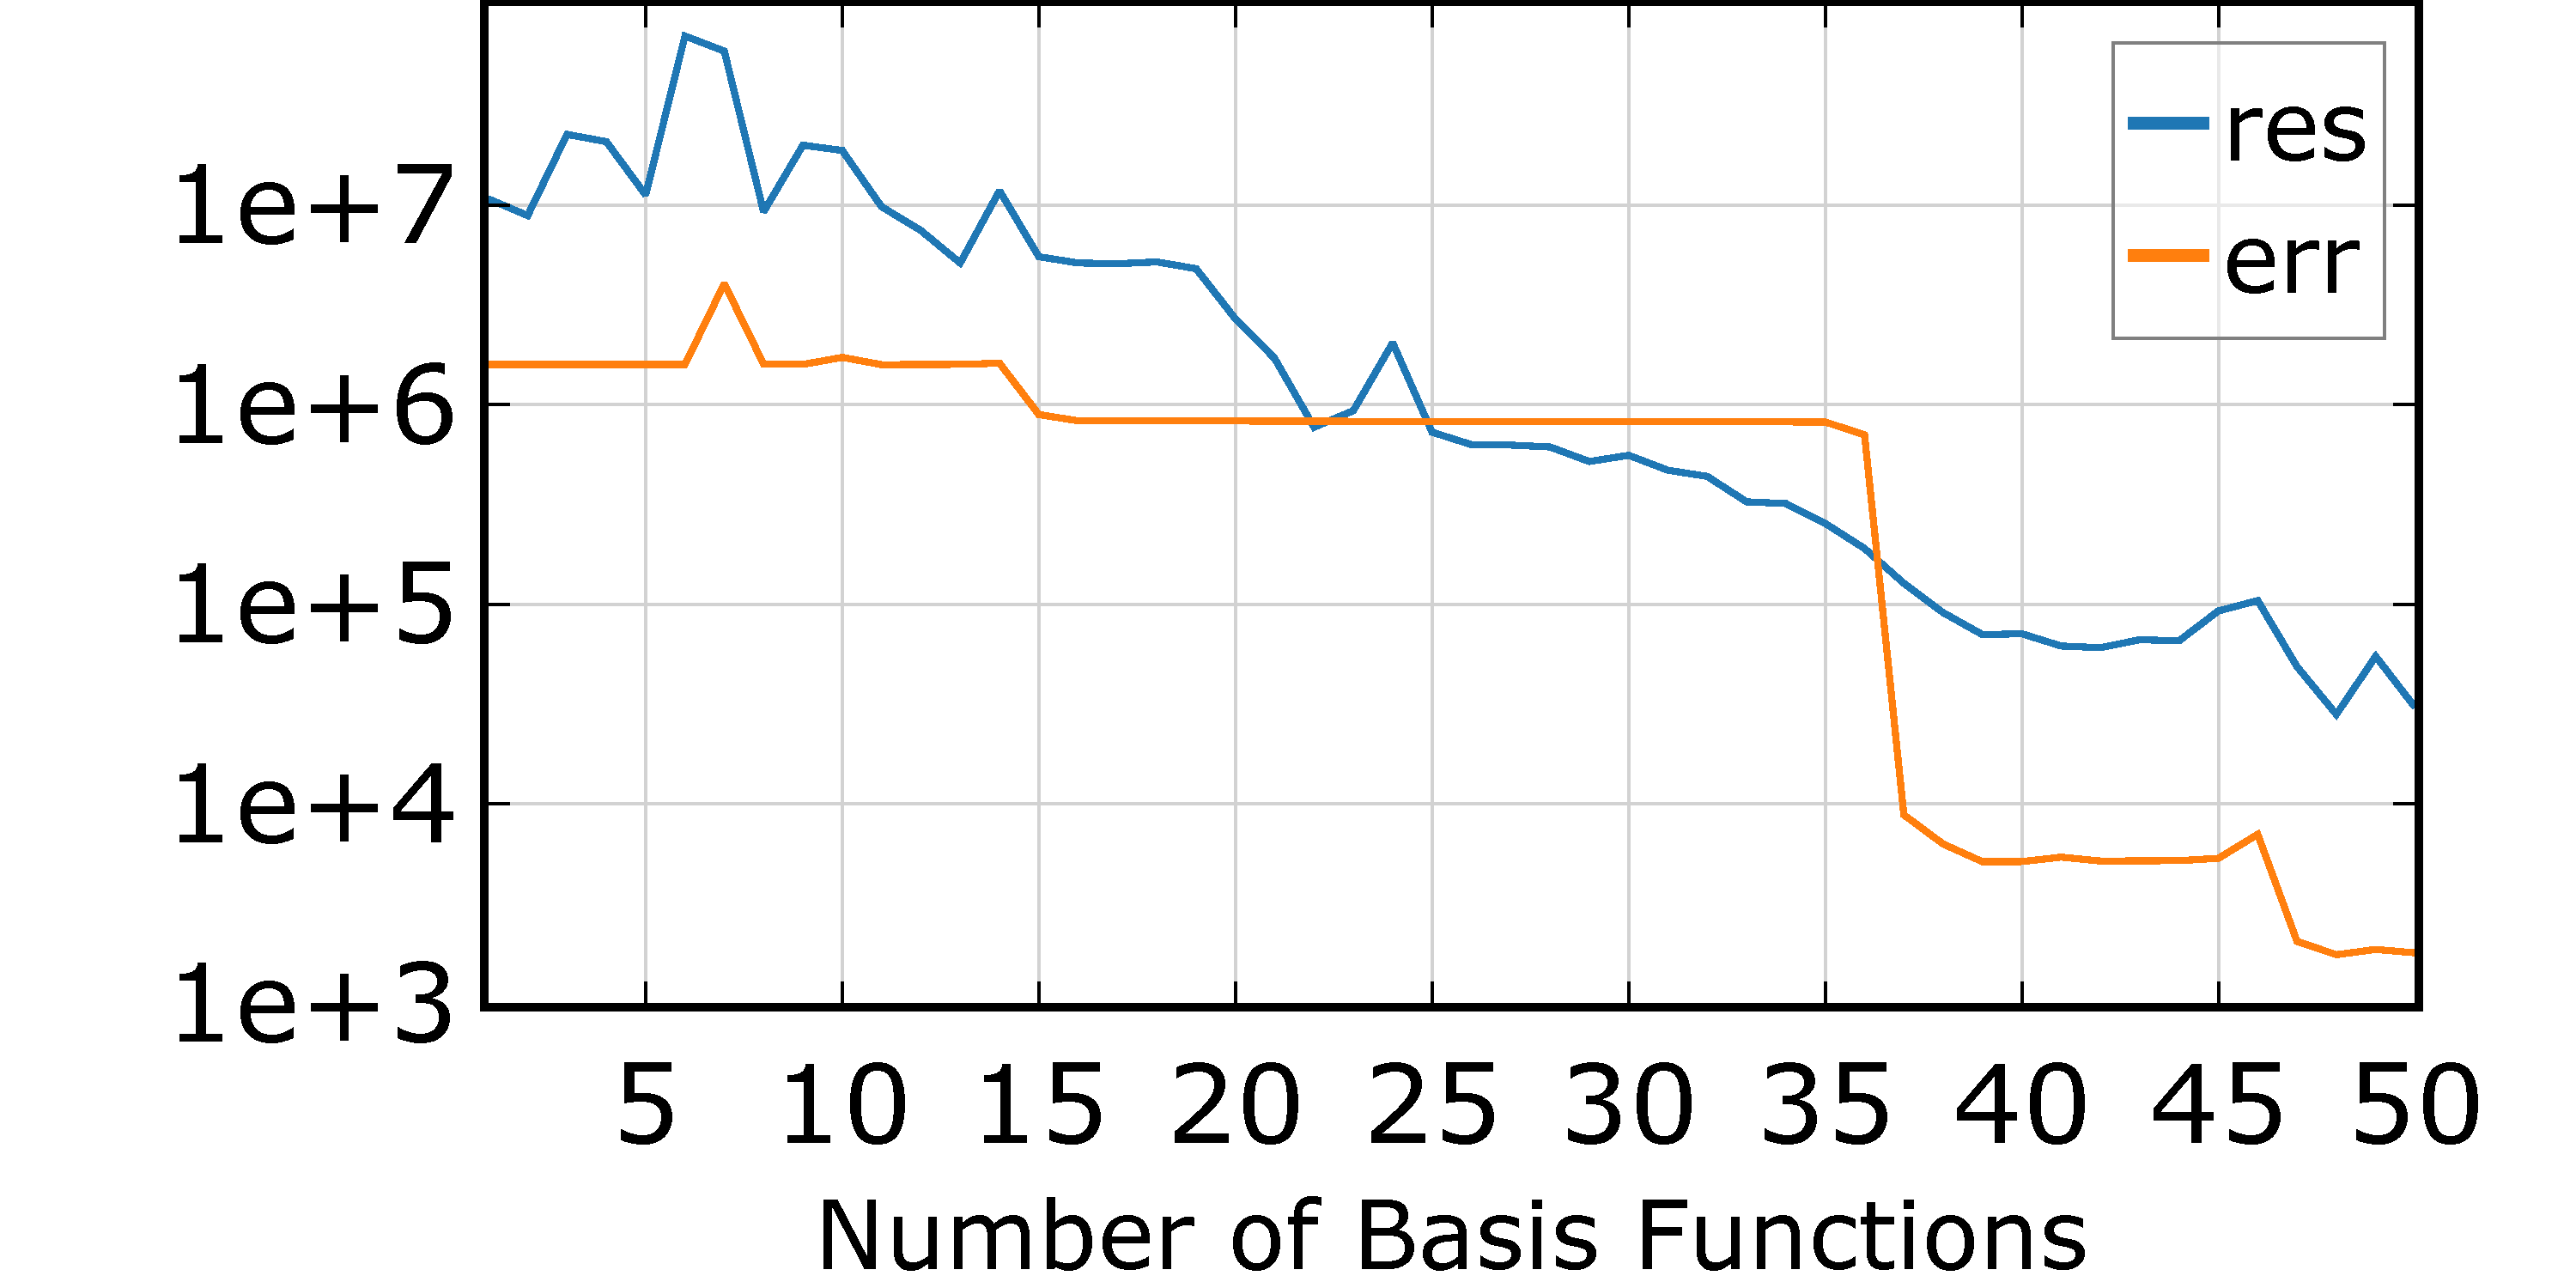
\includegraphics[width=0.5\textwidth]{acc_cav_conv1.pdf}
	\caption{Convergence for the accelerator cavity with the 20.5k node mesh. The sudden drop of the err corresponds to the "finding" of the last resonance.}
	\label{ }
\end{figure}

\begin{figure}[h]
	\centering
	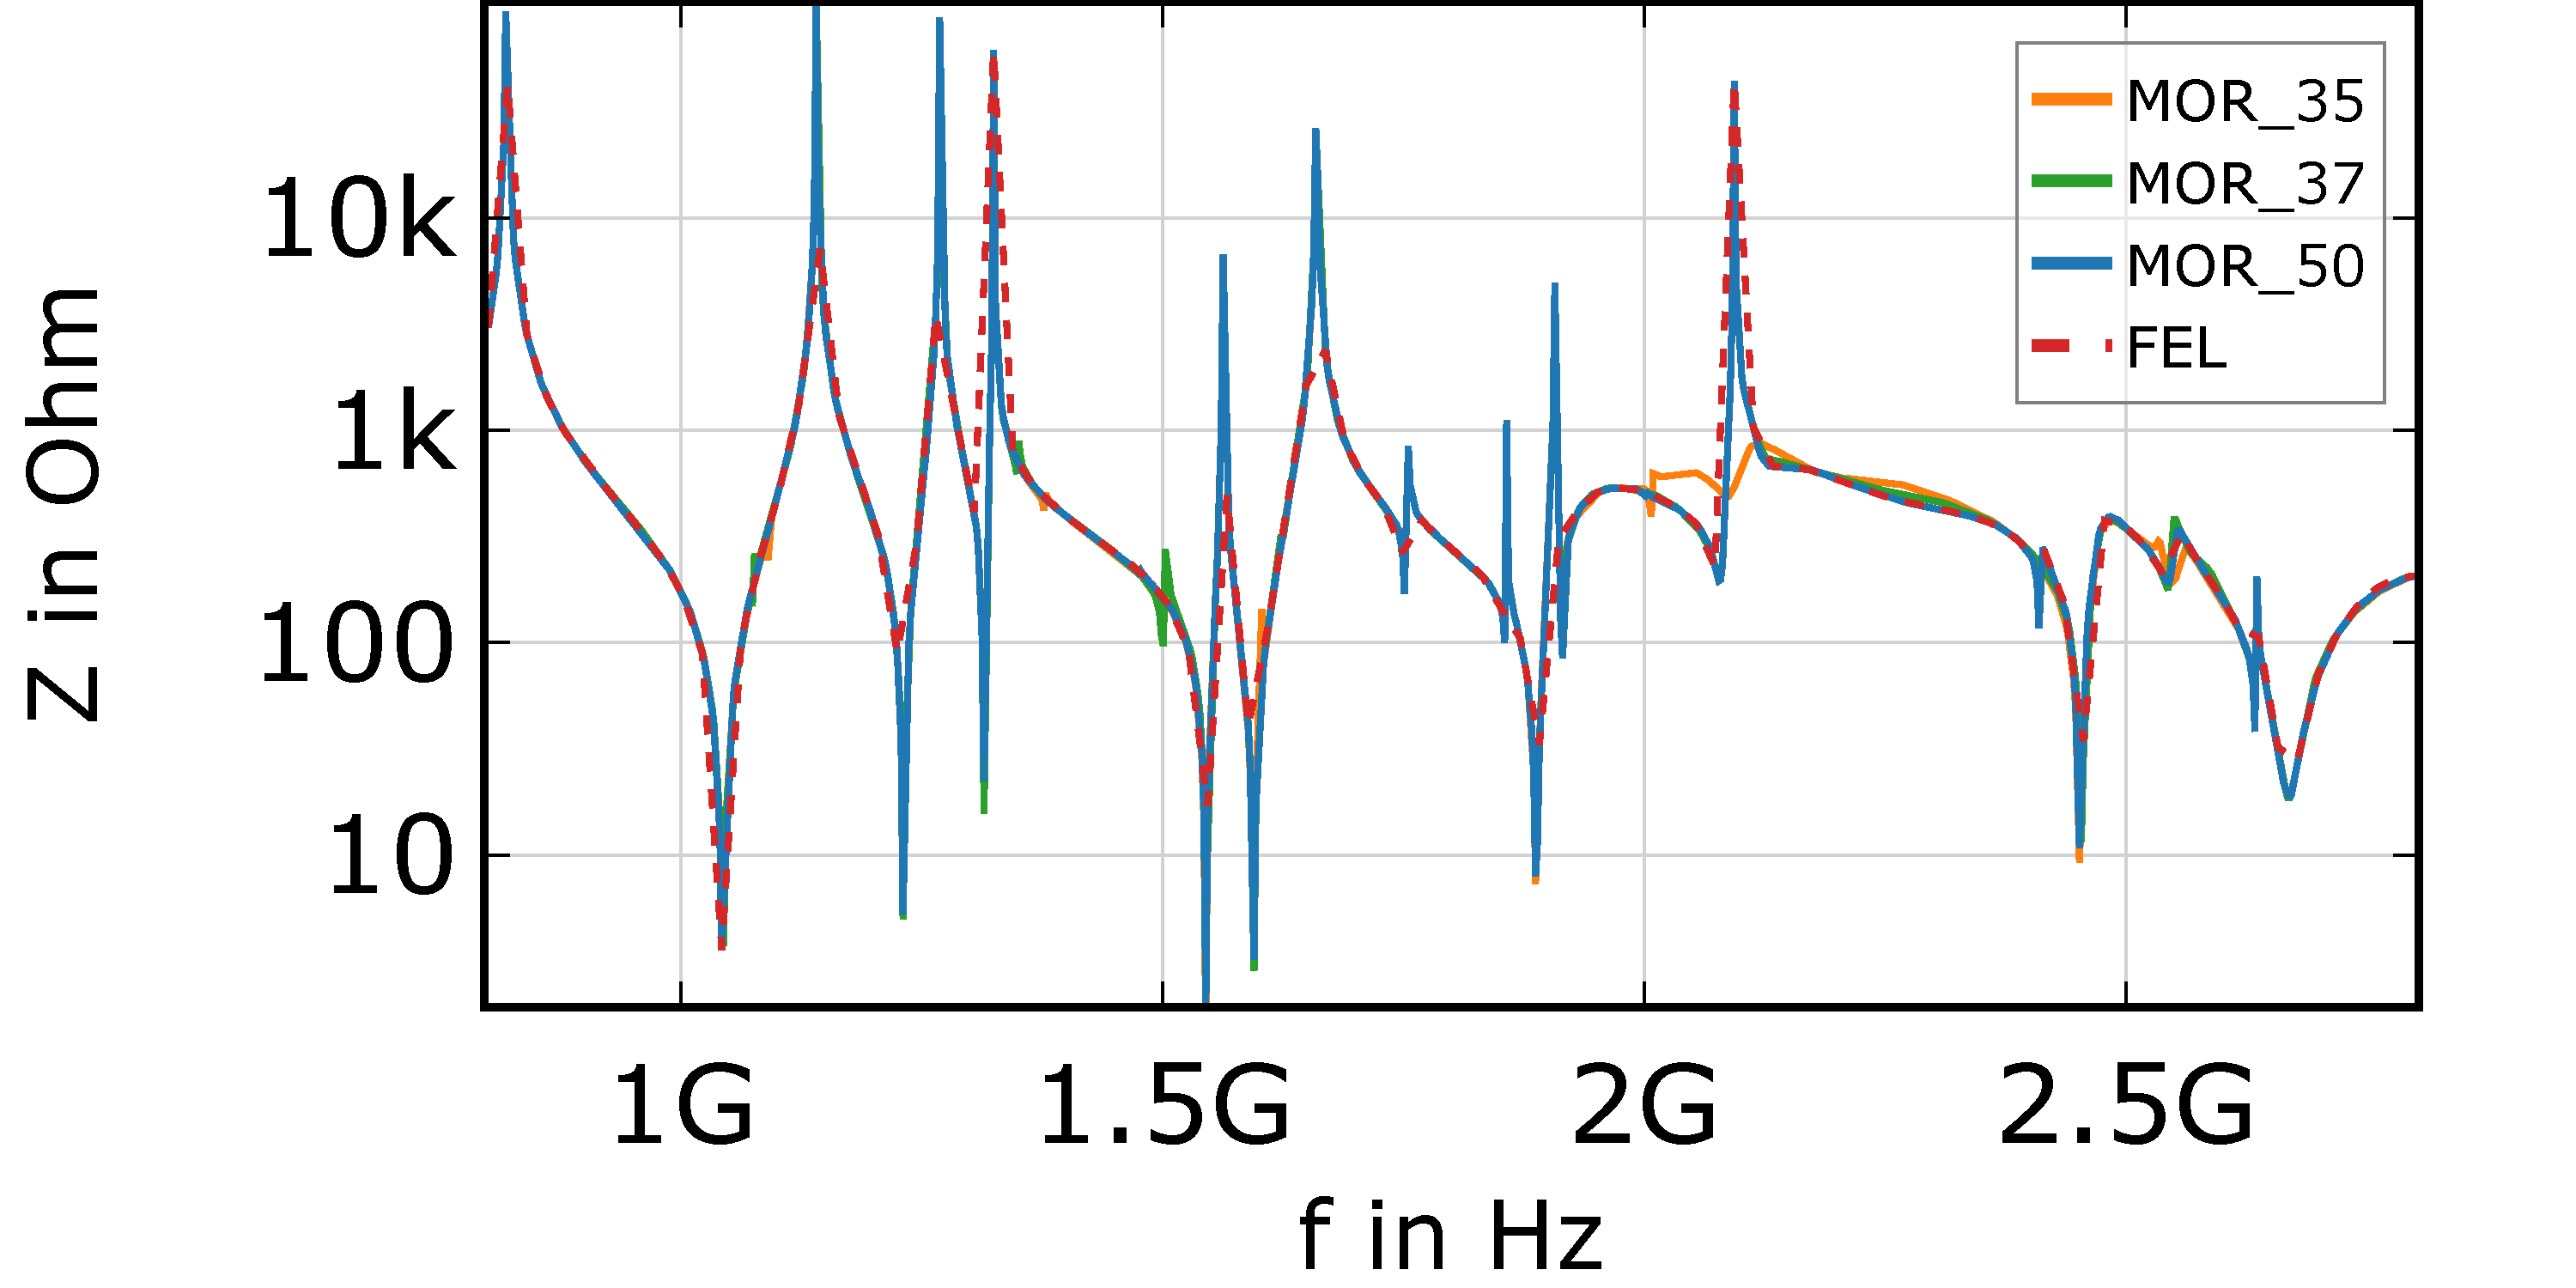
\includegraphics[width=0.5\textwidth]{acc_cav_imp1.pdf}
	\caption{Impedance for the accelerator cavity with the 20.5k node mesh.}
	\label{ }
\end{figure}

\begin{figure}[h]
	\centering
	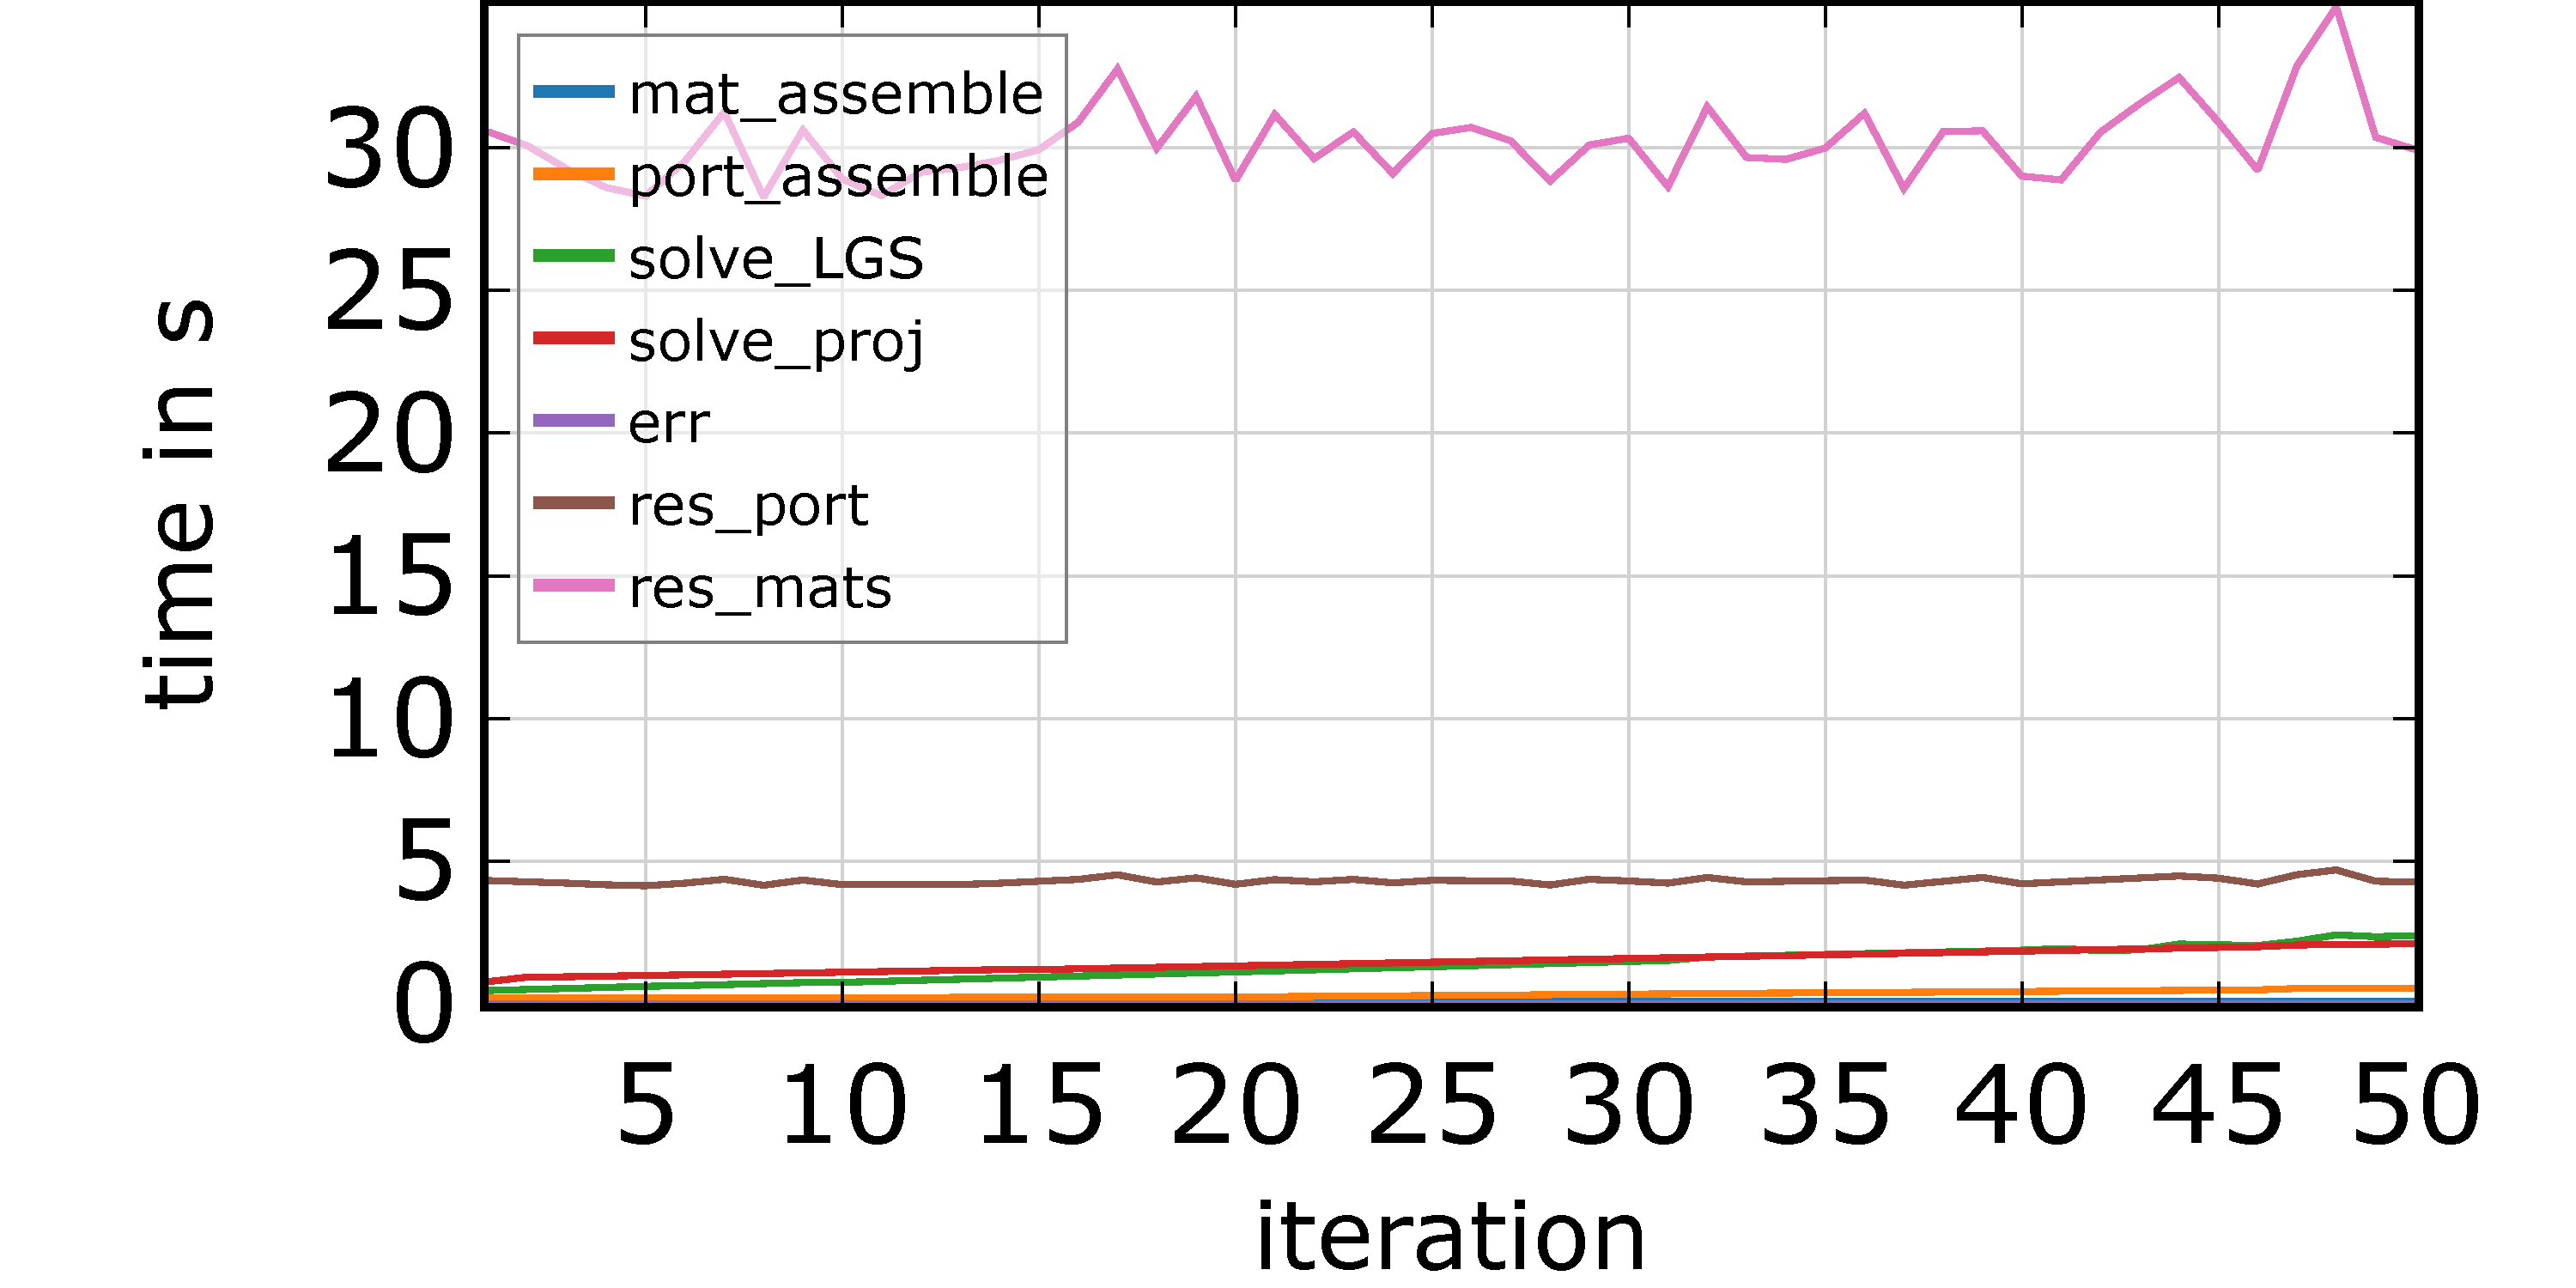
\includegraphics[width=0.5\textwidth]{acc_cav_time1.pdf}
	\caption{Runtime for the accelerator cavity with the 20.5k node mesh. Evaluating the model with FELIS in 100 points took 545s, so 1000 evals would be 5450s. The MOR needed 2774s to reach about 0.2\% of the original residual. Both FELIS and the MOR require about 1GB of memory.}
	\label{ }
\end{figure}

































